\chapter[\hspace{0pt}相关研究技术与理论]{{\heiti\zihao{3}\hspace{0pt}相关研究技术与理论}}

\removelofgap
\removelotgap

本章内容共分为六节,\hyperref[section2: 数字病理图像多实例学习]{第一节}详细介绍病理图像分类任务以及主流的多实例学习架构;
\hyperref[section2: Mamba架构]{第二节}介绍Mamba架构;\hyperref[section2: 对比学习]{第三节}介绍第四章方法应用到的对比学习方法及相关理论;
\hyperref[section2: 数据集及评价指标]{第四节}对本文所使用的数据集和评价指标进行介绍;
\hyperref[section2: 病理图像的预处理过程]{第五节}对病理图像的预处理过程进行详细介绍,\hyperref[section2: 本章小结]{第六节}对本章内容进行总结。

\section[\hspace{-2pt}数字病理图像多实例学习]{{\heiti\zihao{-3} \hspace{-8pt}数字病理图像多实例学习}}\label{section2: 数字病理图像多实例学习}

数字病理图像分类属于前沿且极具潜力的交叉研究领域,它将病理学、图像分析和计算机科学等多学科知识进行深度整合。
此领域借助先进算法、机器学习模型和人工智能技术,以实现对全切片图像(Whole Slide Image,简称 WSI 或病理图像)的全面、精确分析解读,这也是它的核心目标。 
病理图像分类任务通常可分为癌症诊断、亚型分类、生存预测等任务,分别从这些任务角度中辅助病理学家诊断疾病。
数字病理领域,超高分辨率全切片图像(WSI)要完成像素级标注,需投入大量时间与人力。这一难题致使基于像素级标签开展的传统深度学习病理图像分类,难以施展。在此背景下,凭借独特优势,基于多实例学习范式的数字病理图像分类,逐渐成为该领域的常用方法。

多实例学习(Multiple Instance Learning, MIL)~\cite{dietterich1997solving}是弱监督学习的重要分支,其核心思想是处理数据标注在“包”(Bag)级别而非单个实例级别的场景。具体而言,每个数据包包含多个实例,但仅包级别标签已知。经典假设为:若一个包中至少存在一个正实例(Positive Instance),则该包被标记为正类;若所有实例均为负类,则包标记为负类。此范式由Dietterich等人在1997年药物分子活性预测研究中首次提出,并逐渐拓展至计算机视觉、自然语言处理及生物医学等领域。

具体来说,对于在病理图像分类任务而言,一张WSI图像$\mathnormal{X}$将作为一个包,将之切分为多个小图块,将每个图块Patch作为一个实例$x_i$,进而得到实例集合$\mathnormal{X} =\{x_i\}^N_{i=1}$。
需注意,不同包所包含的实例数目$N$并不固定。在任何分类任务里,包$\mathnormal{X}$都附带已知的标签信息$\mathnormal{Y}\in \{0,1\}$,而实例标签$y_i$的具体取值$\{0,1\}$处于未知状态。
以二分类任务为例,包的预测标签\(\mathnormal{Y}\)满足公式:
\begin{equation}
    \mathnormal{Y}=\left \{
    \begin{array}{cl}
        0 &  if \space {\sum_{i}^{N}y_i=0} , \\ 
        1 & otherwise.
    \end{array}\right.
    \label{eq2}
\end{equation} 
而多实例学习模型 $\mathcal{M}(\cdot)$ 的目标是利用所有实例预测包的标签 $\hat{\mathnormal{Y}}\leftarrow\mathcal{M}(\mathnormal{X})$。

早期的方法倾向于预测出每个实例的标签后,再以此推断出包标签。这种方法称之为标签空间级的方法。这类方法非常直观,充分利用了多实例学习的定义,但其实例间关系建模能力有限,且在大规模数据集中面临计算效率瓶颈~\cite{campanella2019clinical} 。鉴于此,当前研究重点逐渐转向特征空间方法,这类方法通过整合包内所有实例的特征信息,构建包的嵌入特征表示,进而实现包级标签的预测。大量的研究证明基于特征空间的方法表现出比标签空间级方法更强的性能。

自Ilse等人\cite{ilse2018attention}提出AB-MIL后,基于注意力的特征空间方法已成为业内主流。该方法通过构建基于上下文感知的注意力机制,动态计算每个实例在包特征嵌入空间中的注意力权重,并据此生成最终的包级特征表示。
例如,DTFD-MIL~\cite{zhang2022dtfd}引入双层多实例学习框架,将图像分割成多个伪包,同样使用注意力机制聚合伪包的预测结果,推断整个病理图像的标签。
Zhu等人~\cite{zhu2024dgr}提出DGR-MIL模型,通过引入可学习的全局向量,精准识别最具代表性的实例,并采用交叉注意力机制计算实例间的重要性,有效挖掘病理图像中的关键特征。
Shao等人~\cite{shao2021transmil}将Transformer架构引入多实例学习框架中,利用空间位置编码保留空间拓扑结构,并通过注意力机制实现实例间关系的多粒度建模。
然而Transformer中自注意力机制计算成本高昂,诸多工作只能采取缩减token数量或采用线性的注意力机制等折中方式将这种复杂模型应用于病理图像分类任务中\cite{tang2024feature}。


\section[\hspace{-2pt}Mamba架构]{{\heiti\zihao{-3} \hspace{-8pt}Mamba架构}}\label{section2: Mamba架构}

Mamba架构是由Albert Gu和Tri Dao等人于2023年提出的新型序列建模框架~\cite{gu2023mamba},其核心创新在于将状态空间模型(State Space Model, SSM)与选择性机制(Selective Mechanism)相结合,
突破了传统Transformer模型在长序列建模中的局限性。该架构通过建立线性时间复杂度与序列长度的关系,显著提升了模型处理长序列依赖的能力,在自然语言处理、基因组学分析、计算机视觉等领域展现出显著优势。

从数学基础来看,Mamba架构以连续时间状态空间模型为理论框架。其核心微分方程可表述为:
\begin{equation}
\begin{aligned}
    h'(t)&=\mathbf{A}h(t)+\mathbf{B}x(t),\\
    y(t)&=\mathbf{C}h(t) +\mathbf{D}x(t),
\end{aligned}
\label{eq3}
\end{equation}
其中$\mathbf{A}$为状态转移矩阵,$\mathbf{B}$、$\mathbf{C}$分别为输入/输出投影矩阵, $\mathbf{D}$为跳跃连接项。通过零阶保持法(Zero-order Hold)的离散化处理,如公式~\ref{eq4}所示:
\begin{equation}
\begin{aligned}
    \mathbf{\bar{A}}&=\exp(\Delta\mathbf{A}),\\
    \mathbf{\bar{B}}&=(\Delta\mathbf{A})^{-1}(\exp(\Delta\mathbf{A})-\mathbf{I})\cdot\Delta\mathbf{B}.
\end{aligned}
\label{eq4}
\end{equation}
模型将连续系统转化为适用于离散序列的递归计算形式,这一过程在保持系统动态特性的同时实现了计算可行性。
与传统递归神经网络不同,Mamba引入了输入依赖的参数动态化机制,通过函数$\mathbf{B},\mathbf{C},\Delta=f_\theta(x_t)$实现参数矩阵的实时生成,使模型能够根据当前输入特征自适应调整状态转移模式。

\begin{figure}[h]
    \centering
    \captionsetup{font={small, stretch=1.312}}
    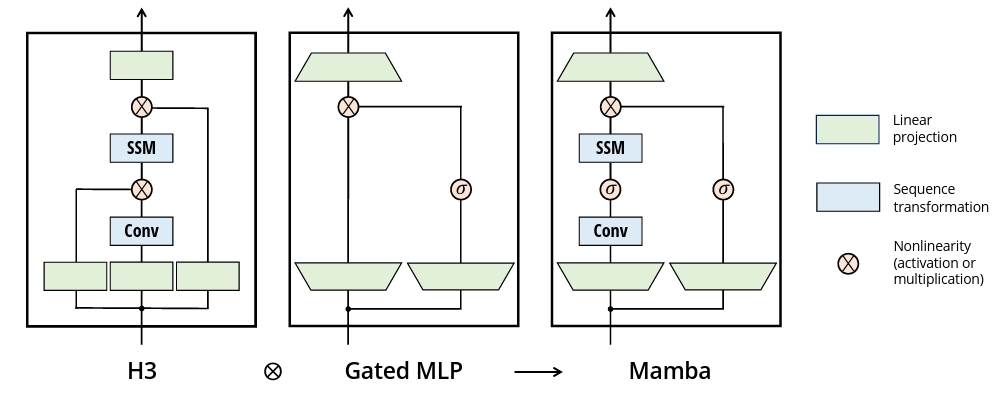
\includegraphics[width=1.0\columnwidth]{figures/RelatedWork/Mamba架构.png}
    \bicaption[Mamba架构示意图]{Mamba架构示意图。~\cite{gu2023mamba}}[Illustration of the Mamba architecture]{ Illustration of the Mamba architecture.~\cite{gu2023mamba}}
    \label{figure1: Mamba架构示意图}
\end{figure}
在架构设计层面,Mamba通过三个关键创新实现突破:首先,提出选择性扫描算法(Selective Scan Algorithm),通过时间步长参数$\Delta$的动态调节,实现高频信号密集采样与低频信号稀疏处理的智能平衡;其次,开发硬件感知并行化技术,利用GPU内存层级特性优化扫描操作的计算模式,在保持线性时间复杂度的同时实现并行加速;最后,采用模块化堆叠结构,通过交替堆叠SSM块与门控前馈网络构建深度模型,配合残差连接和层归一化技术确保梯度有效传播。实验数据显示,在PG19长文本建模任务中,该架构的困惑度相比Transformer降低23\%,训练速度提升5.2倍~\cite{gu2023mamba}。

相较于传统Transformer的 $O(N^2)$复杂度,Mamba在序列长度为N时实现$O(N)$ 的时间与空间复杂度,这一特性使其在万Token级别的高分辨数字病理图像等场景展现独特优势。
但其本质作为序列敏感型模型,对输入实例的排列顺序具有高度依赖性。
这一特性与多实例学习任务中固有的包级序列不变性要求存在根本性冲突,同时也和视觉任务存在偏差,导致模型在病理图像分类等需弱监督定位的关键场景中易受实例顺序扰动影响,制约模型性能的稳定性与可重复性,并影响其在视觉任务更广泛的应用。


\section[\hspace{-2pt}对比学习]{{\heiti\zihao{-3} \hspace{-8pt}对比学习}}\label{section2: 对比学习}

对比学习作为一种自监督学习范式,通过构建正负样本对的差异性建模实现数据表征学习,已经逐渐成为计算机视觉领域的研究热点之一。其核心在于最大化语义相似样本的嵌入相似度,同时最小化不相关样本的关联性。该方法突破了传统监督学习对人工标注的依赖,其表达式如下所示:
\begin{equation}
\label{equation2: infoNCE}
\mathcal{L} = - \text{log}\frac{\text{exp}(cos(f(x), f(x^+)) / \tau)}{\text{exp}(cos(f(x), f(x^+)) + \sum_{j=1}^{N} \text{exp}(cos(f(x), f(x^-))}.
\end{equation}
根据对比学习是否有负样本可以将对比学习分为两类:基于负样本的对比学习、无负样本的对比学习,以下将分别介绍。

\subsection[\hspace{-2pt}基于负样本的对比学习]{{\heiti\zihao{4} \hspace{-8pt}基于负样本的对比学习}}\label{section2: 基于负样本的对比学习}

基于负样本的对比学习方法通过显式地构造负样本对来实现特征判别,代表模型包括SimCLR~\cite{chen2020simple}和MoCo~\cite{he2020momentum}。其核心在于构建动态负样本队列,利用InfoNCE损失函数进行噪声对比估计。
以MoCo v2为例,通过动量编码器(动量系数0.999)维护包含65,536个负样本的特征字典,在ImageNet线性评估协议下达到71.1\%的Top-1准确率~\cite{chen2020improved}。
但该方法面临假负例(False Negative)问题,当负样本中真实正例比例超过5\%时,模型性能下降23\%~\cite{chen2021incremental}

\begin{figure}[h]
    \centering
    \captionsetup{font={small, stretch=1.312}}
    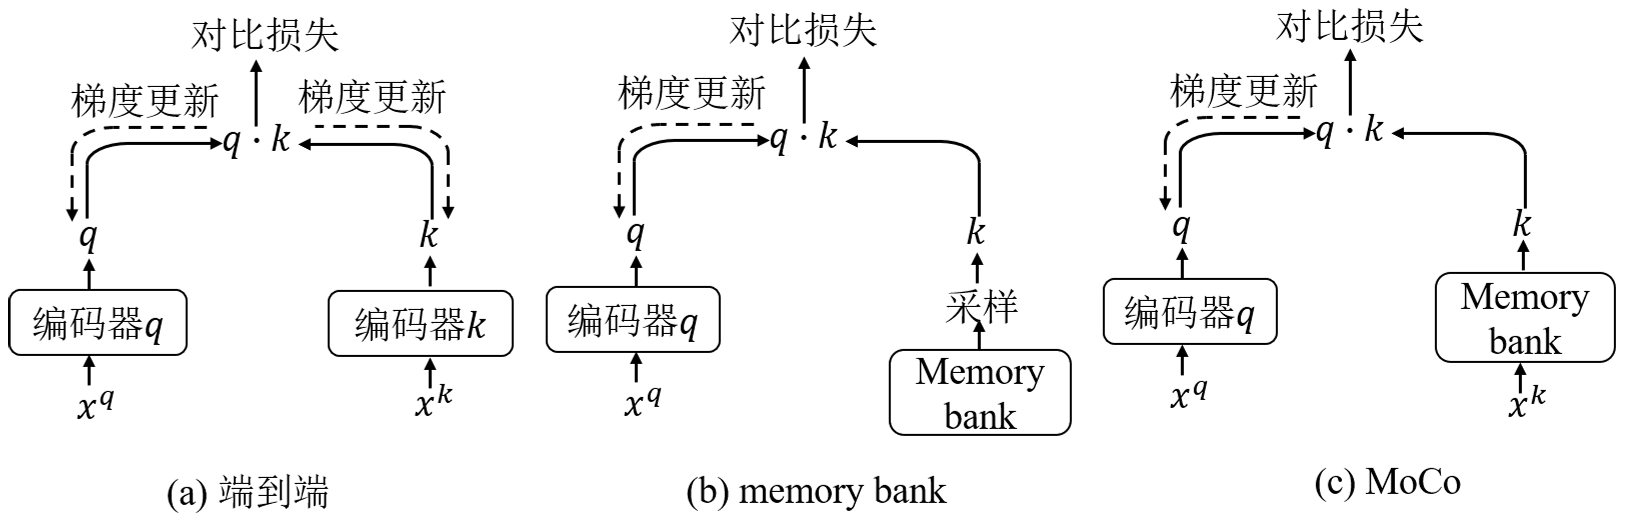
\includegraphics[width=1.0\columnwidth]{figures/RelatedWork/对比学习结构.png}
    \bicaption[对比学习结构示意图]{对比学习结构示意图。}[ Contrastive Learning structure diagram]{ Contrastive Learning structure diagram.}
    \label{figure1: 对比学习结构示意图}
\end{figure}


%其中,图像$x$经由网络$f(\cdot)$后映射到特征空间,$x^+$,$x^-$分别代表$x$的正样本以及负样本,$N$为负样本数量。$cos(\cdot)$是余弦相似度,$\text{exp}(\cdot)$为以e为底的指数函数。

%Chen等人\cite{SimCLR}提出了一个简单有效的无监督对比学习框架-SimCLR,旨在通过比较不同视角下图像的特征表示来学习强大的特征提取网络。SimCLR的核心思想是利用数据增强来产生正样本对,即从同一张图像中通过随机的数据增强操作(如裁剪、颜色变换等)生成两个视角,然后使来自同一图像的特征相互靠近,同时使得来自不同图像的特征尽可能地远离。尽管SimCLR在无监督特征学习方面取得了显著的成果,但其有一个明显缺点,即SimCLR的效果很大程度上依赖于对比损失函数中大量不同的负样本对,为了达到最佳性能,需要批次大小很大,这对计算资源的要求较高。He等人\cite{MoCo}提出的MoCo算法通过引入一个动态字典来存储样本特征表示解决了此问题。这个字典是一个队列,新的样本特征进入队列时,旧的样本特征被移除,以保持队列的固定大小。MoCo可通过此字典高效地采样大量负样本,因此不再需要使用很大的批次便可达到最佳效果。这些无监督对比学习方法特别适合于数据量大但未标注的场景,能够有效地利用大量未标注数据来学习有意义的特征表示。

% 通过无监督对比学习,模型能够捕捉到数据的内在结构和丰富的特征信息,这为后续的监督学习任务,如分类、检测等,提供了强大的预训练模型。此外,该方法也在自然语言处理、图数据分析等领域展现出了广泛的应用潜力。

\subsection[\hspace{-2pt}无负样本的对比学习]{{\heiti\zihao{4} \hspace{-8pt}无负样本的对比学习}}\label{section2: 无负样本的对比学习}

为解决负样本偏差问题,BYOL~\cite{grill2020bootstrap}等框架摒弃负样本依赖,采用非对称网络架构进行自蒸馏学习。
通过在线编码器(Online Encoder)与目标编码器(Target Encoder)的交互更新,结合预测头(MLP Projector)实现特征一致性约束。
实验表明,在ImageNet数据集上,BYOL使用ResNet-50骨干网络可达到74.3\%的线性分类准确率,且对批处理大小敏感性降低80\%。
但该方法需严格防止模型坍塌(Model Collapse),通常需保留BatchNorm层作为隐式正则化器。



\section[\hspace{-2pt}数据集及评价指标]{{\heiti\zihao{-3} \hspace{-8pt}数据集及评价指标}}\label{section2: 数据集及评价指标}

病理图像分类任务通常可分为癌症诊断、亚型分类、生存预测等任务。
从计算机视觉视角来看,癌症诊断本质上是图像二分类任务;癌症亚型分类,属于图像多分类范畴;而癌症生存预测,对应图像回归预测任务。接下来这一节,将围绕这三项子任务,对相关数据集、模型评估指标等展开介绍 。

\begin{table}[h!]
\small    % 设置表格字体为5号
\setstretch{1.245}        % 设置具有指定弹力的橡皮长度(原行宽的1.2倍)
\captionsetup{font={small, stretch=1.512}}
\centering\bicaption[癌症诊断、分型病理图像数据集详情]{癌症诊断、分型病理图像数据集详情。\# 代表具体数目}[Cancer diagnosis, classification WSI dataset details]{Cancer diagnosis, classification WSI dataset details. \# denotes the number of it.}    % 中英文标题
\begin{tabularx}{\textwidth}{lC@{}C @{\hspace{2pt}}C@{\hspace{2pt}}C@{\hspace{2pt}}C}
\toprule
数据集 & \# 病例 & \#WSI & \# 平均图块 & \# 最大图块 & \#最小图块 \\
%\cline{2-5}
%& \raisebox{-2pt}{训练集} & \raisebox{-2pt}{验证集} & \raisebox{-2pt}{测试集} & \raisebox{-2pt}{总数} \\
\midrule
CAMELYON & 370 & 899 & 8108 & 44402 &140 \\
TCGA-NSCLC & 956 & 1053 & 10302 & 43637 &85 \\
TCGA-BRCA & 1062 & 1131 & 8746 & 36618 &283 \\
BRACS     & 189  & 547 & 8429 &  22020 & 106 \\
\bottomrule
\end{tabularx}
%\vspace{-20pt}
\label{table2: dataset1}
\end{table}


\begin{table}[h!]
    \small    % 设置表格字体为5号
    \setstretch{1.245}        % 设置具有指定弹力的橡皮长度(原行宽的1.2倍)
    \captionsetup{font={small, stretch=1.512}}
    \centering\bicaption[生存预测病理图像数据集详情]{生存预测病理图像数据集详情。\# 代表具体数目}[Survival prediction Pathology image dataset details]{Survival prediction Pathology image dataset details. \# denotes the number of it.}    % 中英文标题
    \begin{tabularx}{\textwidth}{lC@{}C @{\hspace{2pt}}C@{\hspace{2pt}}C@{\hspace{2pt}}C}
    \toprule
    数据集 & {\# 病例} & \# WSI & \# 平均图块 & \# 最大图块 & \#最小图块 \\
    %\cline{2-5}
    %& \raisebox{-2pt}{训练集} & \raisebox{-2pt}{验证集} & \raisebox{-2pt}{测试集} & \raisebox{-2pt}{总数} \\
    \midrule
    TCGA-LUAD & 478 & 541 & 10629 & 45783 &85 \\
    TCGA-LUSC & 478 & 512 & 10395 & 33594 &158 \\
    TCGA-BLCA & 376 & 457 & 14364 & 34174 &414 \\
    \bottomrule
    \end{tabularx}
    %\vspace{-20pt}
    \label{table2: dataset2}
    \end{table}



\subsection[\hspace{-2pt}数据集]{{\heiti\zihao{4} \hspace{-8pt}数据集}}\label{section2: 数据集}

\textbf{\textcircled{1}癌症诊断数据集}

\textbf{CAMELYON-16}~\cite{bejnordi2017diagnostic}与\textbf{CAMELYON-17}~\cite{bandi2018detection}作为当前开放获取规模最大的乳腺癌淋巴结转移病理诊断基准数据集,均提供病灶转移状态的二元分类标注(转移/非转移)。
其中,CAMELYON-16数据集的训练集包含由荷兰拉德堡德大学医学中心及乌德勒支大学医学中心联合提供的270张全切片数字病理图像(Whole Slide Image, WSI),并配备独立划分的129张官方测试样本。
CAMELYON-17数据集则进一步整合荷兰五所医疗机构的病理资源,共收录1000张经过专业标注的WSI影像。
考虑到CAMELYON-17官方测试集500张样本的标注信息尚未开放,本研究仅采用其已公开的500张训练样本(对应100个临床病例及其影像学诊断结论)。
尽管不少研究,如文献~\cite{li2021dual,shao2021transmil,tang2023multiple,tang2024feature},采用CAMELYON-16~\cite{bejnordi2017diagnostic}数据集,对不同模型在癌症诊断任务中的性能展开评估。
然而,该数据集仅包含 400 张病理图像,图像数量的局限性,削弱了评估结果的有效性。鉴于此,本文参照 CLAM~\cite{lu2021data}的设置,将CAMELYON-16 与 CAMELYON-17 数据集整合,
最终形成包含370个病例、899张有效样本(阴性样本591例,阳性样本308例)的融合数据集。经预处理后,所有病理图像在20倍光学放大倍率下完成分块处理,单张WSI平均生成8108个有效图像块。

\textbf{\textcircled{2}亚型分型数据集}

TCGA肺癌数据集(\textbf{TCGA-NSCLC})是由美国国家癌症研究所(NationalCancerInstitute, NCI)开发的癌症数据共享系统(The Cancer Genome Atlas, 简称TCGA)。
TCGA包括肺鳞状细胞癌(TCGA-LUSC)和肺腺癌(TCGA-LUAD)两类数据,TCGA-LUSC的 478个病例中有512个WSI,
TCGA-LUAD 478个病例中有541个WSI,共1053个WSI。该数据集仅给出了图像级别的标签。和CAMELYON数据集相比,它的阳性样本中肿瘤区域明显大很多。
TCGA 数据集采用了跟 CAMELYON 数据集一样的数据预处理方法。经过处理后,每一幅放大 20 倍的图像大概能产生 10300 个图像块。TCGA 数据集仅仅提供了图像类别的标注信息,并没有提供细致的像素标注内容。

浸润性乳腺癌数据集(Invasive Breast CCarcinoma, \textbf{BRCA})是肿瘤基因组图谱大型国际研究项目(TCGA)的一个子项目,致力于了解和研究乳腺癌(BRCA)的基因组特征。BRCA项目系统地收集了来自不同乳腺癌患者队列的肿瘤样本,包括原发肿瘤和转移瘤,以及正常对照组织样本(如非癌乳腺组织)。其中浸润性导管癌(IDC) 779张,浸润性小叶癌(ILC) 198张。

\textbf{BRACS}~\cite{brancati2022bracs}是一个同时用于粗粒度和细粒度分型的乳腺癌亚型数据集。其建立在帕斯卡尔基金会(IRCCS Fondazione Pascale)、美国国家研究委员会(National Research Council CNR)的高性能计算与网络研究所(ICAR)和IBM苏黎世研究中心之间的一项协议之上,该协议旨在“通过组织学图像的自动分析来识别乳腺癌病理学中的非典型肿瘤的方法和工具的开发”。在粗粒度的BRACS分型任务中,每个WSI可分为良性(Benign)、非典型(Atypical)和恶性肿瘤(Malignant)。在细粒度的BRACS分型任务中,将每一种WSI分为正常(Normal)、病理良性(Pathological Benign, PB)、普通型导管增生(Usual Ductal Hyperplasia, UDH)、不典型导管增生(Atypical Ductal Hyperplasia, ADH)、扁平上皮不典型(Flat Epithelial Atypia, FEA)、导管原位癌(Ductal Carcinoma in Situ, DCIS)和浸润性癌(Invasive Carcinoma, IC)。其中Normal、PB、UDH被分为良性病灶;FEA、ADH被归类为非典型(Atypical);DCIS和IC被归为恶性肿瘤(Malignant)。BRCAS数据集被官方划分为395个WSIs的训练集、65个WSIs的验证集和87个WSIs的测试集以用于评估。

\textbf{\textcircled{3}生存预测数据集}

癌症预后生存分析的核心,是量化评估患者群体时序生存概率的分布特征,具体涵盖术后存活期预测、复发风险分层及生存状态演化建模等临床关键维度。
本研究选取TCGA数据库中肺腺癌(\textbf{TCGA-LUAD})、肺鳞癌(\textbf{TCGA-LUSC})及膀胱尿路上皮癌(\textbf{TCGA-BLCA})三个项目的临床随访数据构建愈后预测模型。
需要特别说明的是,与上文所述诊断及分型任务不同,生存预测模型以独立病例为最小分析单元:
TCGA-LUAD与TCGA-LUSC项目沿用分型研究中的原始影像数据,但重新构建了包含生存时间、复发状态等临床终点的标注体系;
TCGA-BLCA数据集则专门收录376例膀胱尿路上皮癌(Bladder Urothelial Carcinom)患者的完整临床随访记录。
在实验设计层面,通过整合多中心临床数据构建生存分析框架,重点考察模型对患者个体化生存曲线的预测效能。

\subsection[\hspace{-2pt}评价指标]{{\heiti\zihao{4} \hspace{-8pt}评价指标}}\label{section2: 评价指标}

在癌症诊断与分型分类模型的性能评估中,本研究仿照相关文献~\cite{tang2024feature,tang2023multiple},采用标准化的评价指标体系。
基于分类任务的特征差异,分别选用准确率、ROC曲线下面积(AUC)及F1分数作为核心评估参数:
针对具有二分类特性的肿瘤诊断问题,采用二元F1分数(F1-binary)进行量化分析;而对于涉及多类别判别的癌症亚型分类任务,则选用宏观F1分数(F1-macro)作为评价基准。
AUC 对类别分布不均衡具有较强鲁棒性,且对分类决策阈值变化具有较低敏感性,能够有效量化模型的分类效能。鉴于上述优势,本研究将 AUC 作为核心评价指标,并在消融实验环节着重分析模型的AUC 表现。

在生存预测任务中,本研究依据文献~\cite{yao2020whole,chen2021multimodal,zhou2023cross,wulczyn2020deep,zhu2017wsisa}的设置,选取一致性指数(Concordance Index, C-index)~\cite{harrell1996multivariable}作为生存分析模型的核心评估指标。
该指标在继承AUC评估特性的基础上,针对生存数据特有的删失(censored data)问题进行了算法扩展,可系统评估模型的判别效能——即通过个体风险评分对生存时间进行可靠排序的能力。其数学表达式如\ref{equation3}所示:
\begin{equation}
    \text{C-index} = \frac{
        \sum_{i \neq j} \delta_j \cdot I(T_i < T_j) \cdot I(\hat{S}_i > \hat{S}_j)
    }{
        \sum_{i \neq j} \delta_j \cdot I(T_i < T_j)
    },
    \label{equation3}
    \end{equation}
其中$T_j$表示样本$j$的实际生存时间,$\hat{S}_j$为模型预测的生存概率,${\delta}_j\in \{0,1\}$ 为事件状态指示器($\delta=1$表示发生终点事件)。指示函数$I(\cdot)$在条件成立时取1,否则为0。该计算架构通过约束条件${\delta}_j=1$,确保仅纳入实际发生事件的样本对进行统计评估,从而提升结果的可信度。指标取值范围具有明确临床解释性:当 $\text{C-index}=1$时表征模型具备完全预测能力,而$ \text{C-index}=0.5$则等效于随机猜测。相较于传统AUC指标,C-index的优势在于能够有效处理生存分析中普遍存在的删失数据问题,其评估机制更符合临床研究数据的实际分布特征。

\section[\hspace{-2pt}病理图像的预处理过程]{{\heiti\zihao{4} \hspace{-8pt}病理图像的预处理过程}}\label{section2: 病理图像的预处理过程}

本研究针对数字病理图像高分辨率特性(1-10亿像素)带来的计算挑战,采用多阶段预处理框架实现高效特征提取(图~\ref{figure1: 数字病理图像的预处理过程示意图})。

\textbf{分割组织。}首先基于Openslide库读取WSI数据,通过多尺度分割策略提取有效组织区域。具体操作是先在 32 倍降采样层级下,将图像转换到 HSV 色彩空间,使用中值滤波对图像边缘进行平滑处理,之后依据饱和度通道阈值生成初始二值掩码;
随后实施形态学闭运算消除微米级孔洞,并通过面积阈值过滤非组织区域~\cite{lu2021data}。
为提升算法鲁棒性,系统自动生成包含分割参数及处理日志的元数据文件,支持人工复核与参数微调。

\textbf{划分图块并提取特征。}在20倍光学放大倍率下,采用滑动窗口法从有效组织区域裁剪256×256像素图像块,存储为标准化hdf5格式并记录空间坐标信息。
该尺度选择平衡了细胞形态学特征保留与计算效率,单个WSI可产生10³-10⁴量级图像块(视组织面积而定)。
在特征提取环节,本研究采用了两种特征提取器:其一,采用在 ImageNet 数据集上进行预训练的 ResNet-50 模型~\cite{he2016deep},该模型截断至第三残差块,随后应用自适应均值池化操作,把图像块编码成维度为 1024 的向量;
其二, 在“Mass-100K”上预训练的通用的、用于病理学的自监督视觉编码器UNI~\cite{chen2024towards},同样输出1024维向量。
将提取的特征作为在线深度学习模型监督学习的输入,能大幅缩短训练时间、降低计算成本。基于此构建的特征矩阵,让单个 GPU 在数小时内,就能完成万级全切片图像(WSI)的模型训练。

\begin{figure}[h]
    \centering
    \captionsetup{font={small, stretch=1.312}}
    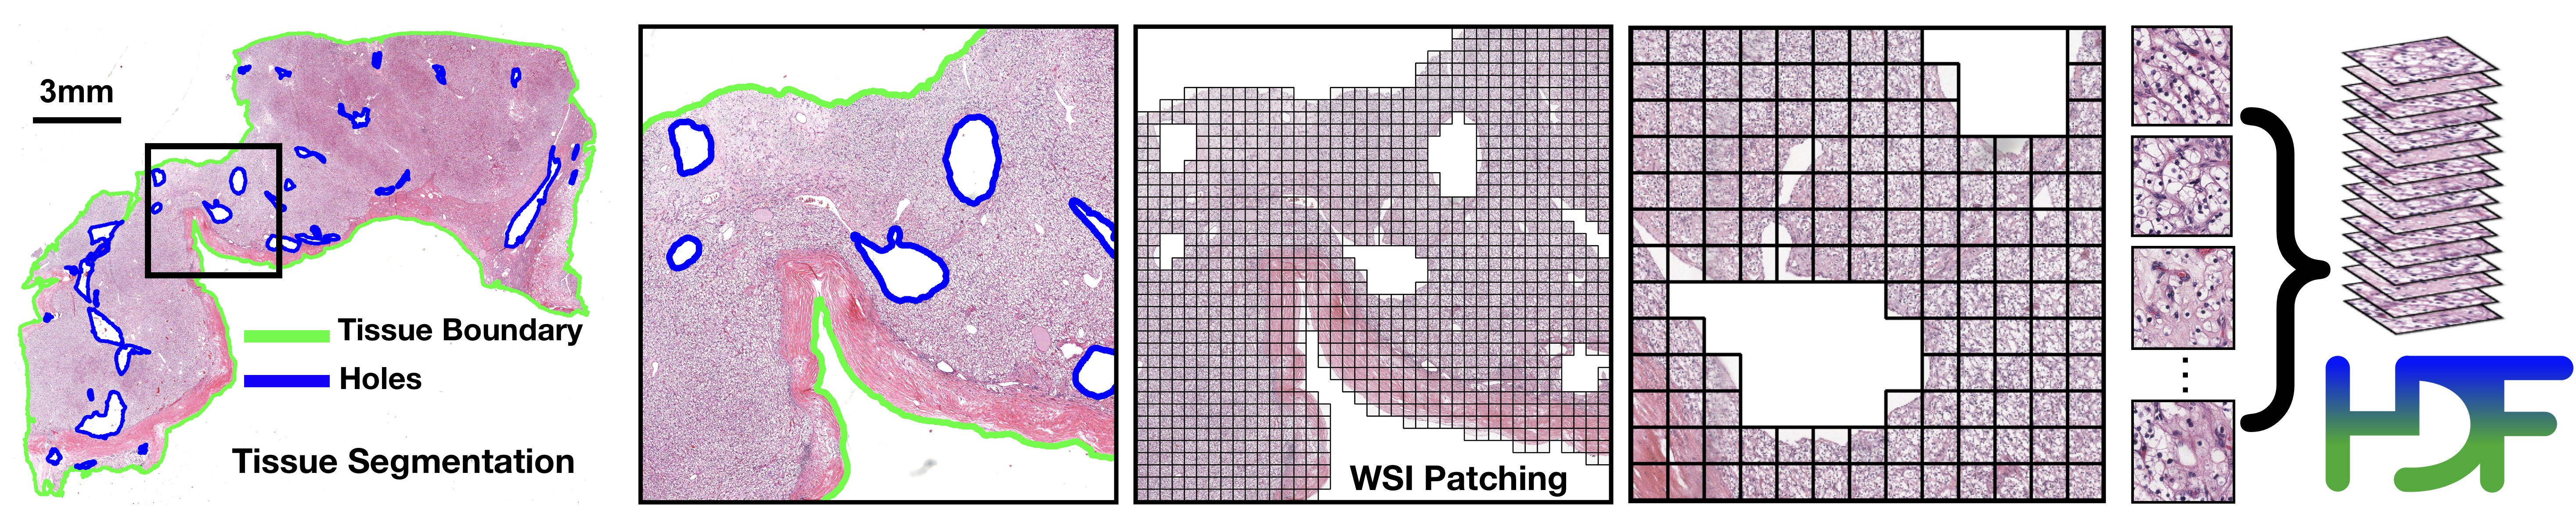
\includegraphics[width=1.0\columnwidth]{figures/RelatedWork/CLAM1.jpg}
    \bicaption[数字病理图像的预处理过程示意图]{数字病理图像的预处理过程示意图。~\cite{lu2021data}}[ Illustration of the WSI preprocessing process]{ Illustration of the WSI preprocessing process.~\cite{lu2021data}}
    \label{figure1: 数字病理图像的预处理过程示意图}
\end{figure}
\section[\hspace{-2pt}本章小结]{{\heiti\zihao{-3} \hspace{-8pt}本章小结}}\label{section2: 本章小结}

本章首先详细介绍病理图像分类常用的多实例学习范式的分类及发展过程,其次介绍了Mamba架构的特点、优势及迁移至视觉领域所面临的挑战。
然后对后续研究工作所涉及到的对比学习等相关技术进行了详细介绍,根据是否使用负样本将其分为基于负样本对比学习和无负样本的对比学习进行了详细阐述。
接着,介绍了本文方法所涉及到的数字病理图像分类子任务、数据集和评价指标等,最后介绍了病理图像的预处理阶段。
